% Construction : h(x) = −0,02x² + 1,3x, la première bissectrice y = x, et
% l'escalier parti de u₀ = 1. Le point fixe est en (15 ; 15) : la suite croît
% en restant sous 20, et s'en approche sans l'atteindre.
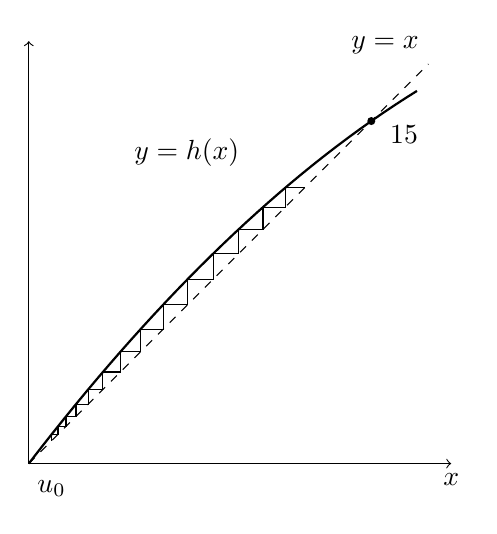
\begin{tikzpicture}[scale=0.29]
  \draw[->] (0, 0) -- (18.5, 0) node[below] {$x$};
  \draw[->] (0, 0) -- (0, 18.5);
  \draw[dashed] (0, 0) -- (17.5, 17.5) node[above left] {$y = x$};
  \draw[thick] plot coordinates {(0.000, 0.000) (0.500, 0.645) (1.000, 1.280) (1.500, 1.905) (2.000, 2.520) (2.500, 3.125) (3.000, 3.720) (3.500, 4.305) (4.000, 4.880) (4.500, 5.445) (5.000, 6.000) (5.500, 6.545) (6.000, 7.080) (6.500, 7.605) (7.000, 8.120) (7.500, 8.625) (8.000, 9.120) (8.500, 9.605) (9.000, 10.080) (9.500, 10.545) (10.000, 11.000) (10.500, 11.445) (11.000, 11.880) (11.500, 12.305) (12.000, 12.720) (12.500, 13.125) (13.000, 13.520) (13.500, 13.905) (14.000, 14.280) (14.500, 14.645) (15.000, 15.000) (15.500, 15.345) (16.000, 15.680) (16.500, 16.005) (17.000, 16.320)};
  \draw (1.000, 1.000) -- (1.000, 1.280) -- (1.280, 1.280) -- (1.280, 1.631) -- (1.631, 1.631) -- (1.631, 2.067) -- (2.067, 2.067) -- (2.067, 2.602) -- (2.602, 2.602) -- (2.602, 3.247) -- (3.247, 3.247) -- (3.247, 4.011) -- (4.011, 4.011) -- (4.011, 4.892) -- (4.892, 4.892) -- (4.892, 5.881) -- (5.881, 5.881) -- (5.881, 6.954) -- (6.954, 6.954) -- (6.954, 8.073) -- (8.073, 8.073) -- (8.073, 9.191) -- (9.191, 9.191) -- (9.191, 10.259) -- (10.259, 10.259) -- (10.259, 11.232) -- (11.232, 11.232) -- (11.232, 12.078) -- (12.078, 12.078);
  \fill (15, 15) circle (5pt);
  \node[right] at (15.4, 14.4) {$15$};
  \node[below] at (1, -0.3) {$u_0$};
  \node[right] at (4.2, 13.6) {$y = h(x)$};
\end{tikzpicture}
